% --- Documentclass specifications ---
\documentclass[italian]{tktltiki2}
\linespread{1.3}

% --- General packages ---
\usepackage[utf8]{inputenc}
\usepackage[T1]{fontenc}
\usepackage{lmodern}
\usepackage{epigraph}
\usepackage{microtype}
\usepackage{amsfonts,amsmath,amssymb,amsthm,booktabs,color,enumitem,graphicx}
\usepackage[pdftex,hidelinks]{hyperref}
% setting C language style listing
\usepackage{listings}
\lstset{
  language=C,
  basicstyle=\fontsize{8}{11}\selectfont\ttfamily
}
% Automatically set the PDF metadata fields
\makeatletter
\AtBeginDocument{\hypersetup{pdftitle = {\@title}, pdfauthor = {\@author}}}
\makeatother

% --- Language-related settings ---
\usepackage[fixlanguage]{babelbib}
% add bibliography to the table of contents
\usepackage[nottoc]{tocbibind}


% --- tktltiki2 options ---
%
% The following commands define the information used to generate title and
% abstract pages. The following entries should be always specified:
\title{%
  \huge Project Heimdall \\
  \large Proposta di implementazione per un web switch \\ 
    concorrente two-way di livello 7 (OSI) con \\
    politiche di bilanciamento del carico stateless e stateful
  }
\author{\emph{Alessio Moretti} - 0187698 \\\emph{Andrea Cerra} - 0167043\\\emph{Claudio Pastorini} - 0186256}
\date{\today}
\level{Corso di Ingegneria di Internet e del Web - A.A. 2014/2015}
\university{\textbf{Università di Tor Vergata}}
\department{\textbf{Ingegneria Informatica}}
\city{Roma}

% If the automatic page number counting is not working as desired in your case,
% uncomment the following to manually set the number of pages displayed in the abstract page:
%
% \numberofpagesinformation{16 pages + 10 appendix pages}

%


\begin{document}

% --- Front matter ---
\maketitle        % title page

\tableofcontents  % table of contents
\pagenumbering{gobble}

% --- Main matter ---
\mainmatter       % clear page, start arabic page numbering

\section{Example section}
% Example of a quote
\begin{quote}
\flushright
	\emph{Yggdrasil, l'albero del mondo, che congiunge i nove regni del cosmo con Asgard, la dimora degli dei.} \\ Heimdall, custode del Bifröst
\end{quote}

% Write some science here
Sample text and a reference\cite{lamport94}. Lorem ipsum dolor sit amet, consectetur adipiscing elit. Donec at lorem varius, sodales diam semper, congue dui. Integer porttitor felis eu tempor tempor. Proin molestie maximus augue in facilisis. Phasellus eros dui, blandit eu nibh ut, pharetra porta enim. Cum sociis natoque penatibus et magnis dis parturient montes, nascetur ridiculus mus. Aliquam ullamcorper risus pretium est elementum, eget egestas lorem fermentum. Etiam auctor nisi purus, vitae scelerisque augue vehicula sed. Ut eu laoreet ex. Mauris eu mi a tortor gravida cursus eget sit amet ligula.

\begin{figure}
\centering

\includegraphics[width=\textwidth]{images/thor}
\caption{Thor di Asgard, \emph{figlio di Odino}}
\end{figure}



\newpage
\section{Introduzione}

\subsection{Perchè Heimdall?}
Heimdall è il personaggio dell'universo Marvel, ispirato all'omonimo dio della mitologia norrena, egli è il guardiano del regno di Asgard e del Bifröst. Quest'ultimo è il ponte che unisce la Terra alla dimora degli dei ed Heimdall, come suo custode, ha il compito di aprirlo ed indirizzarlo verso gli altri mondo, permettendo solamente a chi è degno di attraversare le distese dello spazio. \\
Ci piace pensare che questo sia un po' il ruolo del software nato dal nostro progetto: che sia in grado di scegliere come meglio indirizzare le connessioni in arrivo, ponendosi come 'guardiano' di un cluster di server che fa ad esso capo. Quindi un \textbf{web switch} che sia funzionale sia per ricevere o trasmettere pacchetti di un regolare traffico HTTP che per bilanciare il carico dello stesso traffico in arrivo sulle varie macchine.

\subsection{Web switch di livello 7}
Nella terminologia delle reti informatiche uno \textbf{switch} è un commutatore a livello datalink, ovvero un dispositivo che si occupa di instradare opportunamente, attraverso le reti LAN, selezionando i frame ricevuti e reindirizzandoli verso la macchina appropriata a seconda di una propria tabella di inoltro. Un \textbf{web switch}, a livello applicativo, è capace di reindirizzare i dati in funzione dei pacchetti che riceve, analizzandone il contenuto e decidendo opportunamente la destinazione, occupandosi allo stesso tempo di reinoltrare anche l'eventuale risposta della macchina selezionata verso il client che l'ha generata. \\
Le applicazioni sono molteplici per l'implementazione a livello applicativo: può essere considerato un \textbf{proxy}, oppure, selezionando opportunamente la macchina con più velocità di risposta o con minore pressione, può agire come \textbf{bilanciatore di carico}. Infatti ognuno dei client che fa richiesta, ad esempio, per uno specifico sito web, invia un pacchetto ad un indirizzo IP pubblico che corrisponde a quello del nostro switch applicativo. Questi, dopo aver correttamente letto il pacchetto, si occupa di consultare una tabella di inoltro generata con una determinata \textbf{politica di scheduling} e quindi gestire l'inoltro della richiesta ed il reinoltro della risposta del webserver. tutto questo in maniera totalmente trasparente al client, qualsiasi sia la macchina che ha effettivamente risposto, che sia un web server oppure un cluster di macchine associate ad un ulteriore switch.

\subsection{Assunzioni progettuali sul cluster}
Nella fase di progettazione e realizzazione sono state definite le seguenti assunzioni:
\begin{itemize}
	\item Ognuna delle macchine del cluster dispone di un web server Apache in ascolto sulla porta 80
	\item Ognuna delle macchine monta il modulo ApacheStatus come monitor di carico
\end{itemize}


\begin{figure}
\centering
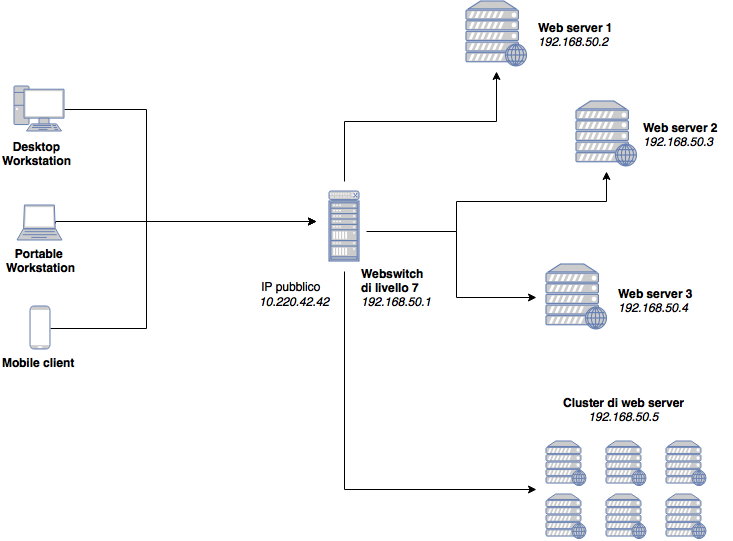
\includegraphics[width=\textwidth]{images/switch7}
\caption{Esempio di uno \emph{switch di livello 7 (OSI)}}
\end{figure}


\newpage
\section{Architettura}

\subsection{Server in ascolto}
\subsubsection{File di configurazione}
\subsubsection{Logging}
\subsubsection{Gestione degli errori}

\subsection{Pool manager}

\subsection{Scheduler} \label{ssec: sched}
Lo scheduler è un componente fondamentale di un sistema informatica: si occupa di stabilire un ordinamento temporale l'esecuzione di un set di richieste di accesso ad una risorsa. Nel caso di un web switch di livello 7, lo scheduler va a garantire che ognuna delle richieste in arrivo possa essere inoltrata immediatamente alla prima macchina disponibile, secondo una politica di scheduling che sia \emph{state-less}, quindi che non consideri l'attuale carico di lavoro delle macchine del cluster, oppure \emph{state-aware}, che monitori costantemente tale carico e modifichi di conseguenza l'assegnazione delle richieste (verrà spiegato nel dettaglio come lavorano e quando sono disponibili tali politiche in \emph{\ref{sec: sched_p}}). \\\\
In questa implementazione lo scheduler, che come vedremo va a sfruttare un algoritmo di selezione \emph{Round Robin} la cui struttura verrà esplicitata più avanti, viene definito come segue.
\begin{lstlisting}
/*
 * ---------------------------------------------------------------------------
 * Structure        : typedef struct scheduler_args
 * Description      : This struct represents the arguments necessary to run the
 *                    scheduler properly
 * ---------------------------------------------------------------------------
 */
typedef struct scheduler_args {
    RRobinPtr     rrobin;                                   // Round Robin struct
    ServerPoolPtr server_pool;                              // Server Pool struct

    ServerPtr (*get_server)(RRobinPtr rrobin);              // to retrieve a server
} Scheduler, *SchedulerPtr;


\end{lstlisting}
In particolare la \textbf{pool dei server} altro non è che un \emph{lista collegata} formata da strutture dati elementari per la gestione dei server indicati nel file di configurazione come appartenenti al cluster, definite come segue
\begin{lstlisting}
/* ---------------------------------------------------------------------------
 * Structure        : typedef struct server_node
 * Description      : This struct represents a single server node in order to
 *                    manage a pool of remote machines
 * ---------------------------------------------------------------------------
 */
typedef struct server_node {
    char *host_address;                                         // machine canonical name
    char *host_ip;                                              // machine ip address
    int  status;                                                // machine status
    int  weight;                                                // machine weight

    struct server_node *next;                                   // next server_node
} ServerNode, *ServerNodePtr;

\end{lstlisting}
mentre le strutture dati che vengono elaborate ed utilizzate come valore di ritorno della schedulazione e che sono alla base della costituzione del buffer su cui opera Round Robin, non sono altro che una versione semplificata e costituita dalle sole informazioni di base per la connessione. \\\\
Nella \textbf{fase di inizializzazione} viene quindi popolata la pool recuperando gli indirizzi delle macchine del cluster, che vengono settate come disponibili e con peso minimo. Quindi a seconda che si sia configurato il web switch in modalità \emph{state-aware} o \emph{state-less}, rispettivamente viene o non viene istanziato un thread che si occuperà di aggiornare periodicamente, con gestione degli accessi concorrenti al buffer del Round Robin, lo stato delle macchine. Ogni volta che una connessione viene accettata viene recuperato un server valido da passare al processo che gestirà la connessione tramite memoria condivisa.
\begin{lstlisting}
\* inside thread pool ... *\
// Retrieving server from scheduler
ServerPtr server = get_scheduler()->get_server(get_scheduler()->rrobin);
// Storing server in shared memory
worker_pool->worker_server[position] = *server;
	
\end{lstlisting}
Viene sempre selezionato un server che sia disponibile, quindi viene sempre effettuato un controllo sullo \emph{status} dello stesso server, nel caso in cui sia abilitato il controllo sullo stato della macchina: l'unico caso in cui questi risulta \emph{BROKEN} e non \emph{READY} è nella circostanza in cui ogni server del cluster risulta non disponibile per cui il worker (che analizzeremo in \emph{\ref{ssec: worker}}) non avvierà nessuna connessione di inoltro della richiesta. \\\\
Dalla necessità progettuale di garantire uno \textbf{scheduling adattabile} a condizioni di stress da carico, quindi per soddisfare specifiche di \emph{state-awareness}, nascono i parametri relativi a status e peso nei nodi della pool di server e nasce un adattamento \emph{pesato} dell'algoritmo di Round Robin.



\subsection{Worker} \label{ssec: worker}
\subsubsection{Gestione delle richieste}
\subsubsection*{Coda delle richieste}
\subsubsection*{Chunk di dati}
\subsubsection{Gestione delle connessioni}
\subsubsection*{Connessione}
\subsubsection*{Richieste HTTP}
\subsubsection*{Risposte HTTP}
\subsubsection{Thread di lettura}
\subsubsection{Thread di scrittura}
\subsubsection{Thread di richiesta}
\subsubsection{Thread di watchdog}

\newpage
\section{Ulteriori proposte}

\newpage
\section{Politiche di scheduling} \label{sec: sched_p}
La schedulazione permette la selezione della macchina predisposta a rispondere alla richiesta HTTP appena arrivata da parte del client, si basa su una tecnica nota come \textbf{bilanciamento del carico}, ovvero la distribuzione del carico, solitamente di elaborazione o di erogazione di uno specifico servizio, tra più server. Questo permette di poter \textbf{scalare} sulla potenza di calcolo del cluster dietro al web switch, lasciando che siano diverse macchine a rispondere a seconda di quella che è più veloce, più performante, oppure monitorando costantemente lo stato dei server e scegliendo quello meno sottoposto ad una pressione del carico di lavoro. Le macchine, specificando hostname ed indirizzi IP, sono date in un apposito file di configurazione.\\\\ 
Nella nostra implementazione \textbf{thread scheduler} si occupa di fornire,  ogni volta che viene invocato, una macchina selezionata secondo una delle due politiche che andremo ora a spiegare nel dettaglio.

\subsection{State-less: implementazione con Round-Robin}
L'algoritmo di scheduling Round-Robin (da adesso RR, \emph{n.d.r.}) è un algoritmo che agisce con prelazione distribuendo in maniera equa il lavoro, secondo una metrica stabilita in partenza. Vediamo quindi la struttura che si occupa di gestire la schedulazione tramite Round-Robin e che contiene le funzioni \emph{wrapper} alle strutture dati che garantiscono il suo corretto funzionamento.\\
\begin{lstlisting}
/*
 * ---------------------------------------------------------------------------
 * Structure        : typedef struct round_robin_struct
 * Description      : This struct represents a Round Robin discipline that can
 *                     be used also a stateful discipline with minimum overhead
 *                    (weighted mode enabled)
 * ---------------------------------------------------------------------------
 */
typedef struct round_robin_struct {
    CircularPtr circular;

    ThrowablePtr (*weight)(CircularPtr circular, Server *servers, int server_num);
    ThrowablePtr (*reset)(RRobinPtr rrobin, ServerPoolPtr pool, int server_num);
    Server *(*get_server)(CircularPtr circular);
}RRobin, *RRobinPtr;

\end{lstlisting}
\begin{figure}[b]
\centering
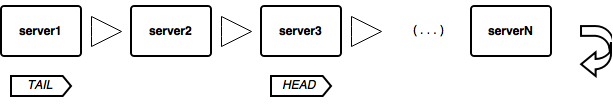
\includegraphics[width=\textwidth]{images/rrobin_stateless}
\caption{Schema di funzionamento del buffer circolare \label{fig: rrobin_sl}}
\end{figure}
Possiamo osservare come siano mantenuti i puntatori alle funzioni necessarie al caso di politica di scheduling \emph{state-aware}, ma per ora l'unica vera funziona a cui si farà accesso è quella per il recupero del server correntemente selezionato. \\\\
L'algoritmo funziona utilizzando un \textbf{buffer circolare} come possiamo vedere in \emph{figura \ref{fig: rrobin_sl}}: questo permette di iterare la selezione su una lista di elementi precedentemente caricata. Possiamo osservare che, oltre alle funzioni e le variabili necessarie a garantire l'accesso atomico all'area di memoria che contiene il buffer, necessario come vedremo nel caso \emph{state-aware} per evitare la concorrenza con il thread che si occupa dell'update dello stato, sono mantenuti:
	\begin{itemize}
  		\item Un puntatore all'array di server 
  		\item La posizione attuale del puntatore di \emph{testa} 
  		\item La lunghezza del buffer, necessaria anche per le operazioni di aggiornamento dei puntatori
  		\item I puntatori di \emph{testa} e \emph{coda} per avanzamento e lettura dal buffer
	\end{itemize}
	Le funzioni restanti permettono di inizializzare il buffer (oltre che di liberare con sicurezza l'area di memoria occupata) e di aggiornare i puntatori sopra menzionati.\\
\begin{lstlisting}
/*
 * ---------------------------------------------------------------------------
 * Structure        : typedef struct circular_buffer
 * Description      : This struct helps to manage a circular buffer of fixed length
 * ---------------------------------------------------------------------------
 */
typedef struct circular_buffer {
    Server      *buffer;
    int         buffer_position;
    int         buffer_len;
    
    Server      *head;
    Server      *tail;

    pthread_mutex_t mutex;

    ThrowablePtr (*allocate_buffer)(CircularPtr *circular, Server **servers, int len);
    ThrowablePtr (*acquire)(struct circular_buffer *circular);
    ThrowablePtr (*release)(struct circular_buffer *circular);
    void         (*progress)(struct circular_buffer *circular);
    void         (*destroy_buffer)(struct circular_buffer *circular);
} Circular, *CircularPtr;

\end{lstlisting}
\break
È necessario quindi specificare tre passi per il corretto funzionamento, dopo aver dato un rapido sguardo alla struttura che lo rappresenta nella nostra implementazione. \\\\
\textbf{Inizializzazione del buffer} in questa fase la struttura dati che rappresenta il buffer circolare, che abbiamo visto mantenere due puntatori di \emph{testa} e \emph{coda}, viene inizializzata associandovi un array di puntatori di strutture di tipo \emph{Server}, precedentemente allocata ed il cui pattern è stato fissato, e viene eseguita la funzione di allocazione del buffer: 
\begin{lstlisting}
    /* inside allocate_buffer ... */
    // allocating the buffer
    circular->buffer = *servers;
    circular->buffer_len = len;
    // setting params
    circular->head = circular->buffer;
    circular->tail = circular->buffer + (len - 1);
    
\end{lstlisting}
In un'ottica di \emph{produttore vs consumatore}, chiaramente visibile nella figura precedente, è necessario che testa e coda non coincidano mai per evitare concorrenza. In questa implementazione si è deciso di separare l'accesso concorrente alla struttura, per il suo aggiornamento, e la lettura dei dati in essa contenuti. Quindi la \emph{testa} conterrà il puntatore al prossimo server da selezionare per schedulare la richiesta, mentre la \emph{coda} punterà all'area di memoria contenente il server attualmente selezione per la schedulazione. \\\\
\textbf{Aggiornamento dei puntatori} per poter sfruttare le peculiarità di questa struttura dati è necessario che i due puntatori vengano aggiornati secondo l'aritmetica del buffer circolare per cui, una volta raggiunta l'estremità dell'array, il valore successivo della posizione corrente ritorna ad essere quello del primo valore dello stesso array. \\
Nel dettaglio viene eseguito, secondo le specifiche sopra riportate, nella nostra implementazione, la seguente funzione:
\begin{lstlisting}
void progress(CircularPtr circular) {
    // recomputing tail, head and buffer position
    circular->tail            = circular->head;
    circular->buffer_position = (circular->buffer_position + 1) % circular->buffer_len;
    circular->head            = circular->buffer + circular->buffer_position;
}

\end{lstlisting}
\textbf{Selezione del server} a questo punto, una volta che il thread chiamante invoca lo scheduler per recuperare il server che è stato selezionato dall'algoritmo, lo scheduler a sua volta invoca la funzione wrapper dalla struttura che gestisce la politica RR e questa esegue il codice ora riportato.
\begin{lstlisting}
    /* inside get_server ... */
    // allocating server ready struct
    ServerPtr server_ready = malloc(sizeof(Server));
   
    /* ... */
    
    // stepping the circular buffer
    circular->progress(circular),
    // retrieving server from tail 
    *server_ready = *(circular->tail);
    return server_ready;
    
\end{lstlisting}
In conclusione quello che stiamo attuando è un \textbf{bilanciamento del carico uniforme} su ognuna delle macchine del cluster. Infatti, senza condizioni sullo stato delle macchine, iterando semplicemente sull'array dei server, ad ogni nuova connessione verrà assegnata una macchina diversa, alleggerendo tutti i server e pareggiando per ciascuno il carico. Il cluster manterrà il carico complessivo ma ogni singola unità contribuirà equamente a soddisfare le connessioni in arrivo.
\newpage
\subsection{State-aware: implementazione con monitor di carico}

\begin{figure}[t]
\centering
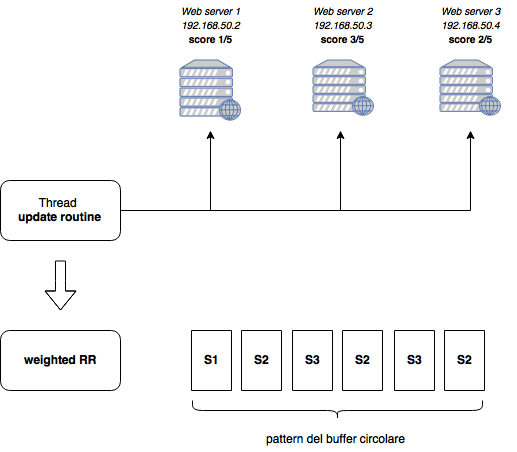
\includegraphics[width=\textwidth]{images/rrobin_stateaware}
\caption{Schema della procedura di aggiornamento dello stato dei server \label{fig: rrobin_sa}}
\end{figure}

Un algoritmo di schedulazione cosiddetto \emph{state-aware} si occupa di selezionare la macchina a cui inoltrare la connessione basandosi non solo sulla conoscenza delle macchine presenti nel cluster ma anche sul loro status. In particolare, in questa implementazione, si è deciso di ricorrere all'analisi dei risultati di un \textbf{monitor di carico} presente su ciascuna delle macchine del cluster (in riferimento alle assunzioni progettuali, questi è i modulo \emph{ApacheStatus} di cui si parlerà più avanti in \emph{\ref{sssec: apachestatus}} ). Tale monitor, che ritorna una serie di parametri indici dell'attuale impiego di risorse della macchina, permette di definire un \textbf{algoritmo pesato} per la selezione del server che risponderà alla connessione in arrivo al web switch. \\
Anche in questo caso andremo a determinare una serie di passi che vengono seguiti, tenendo conto che in fase progettuale \emph{si è deciso di sfruttare lo stesso algoritmo RR} già utilizzato nel caso \emph{state-less}, ma che ricordiamo essere stato predisposto per una ulteriore versione pesata. Per far questo si lavora sulla struttura Server \\\\
\textbf{Detachment del thread di update} nei file di configurazione dell'applicazione è possibile definire due livelli di lavoro:
	\begin{itemize}
		\item \textbf{AWARENESS\_LEVEL\_LOW} che corrisponde ad una versione state-less dell'algoritmo RR e si riporta al caso precedente
		\item \textbf{AWARENESS\_LEVEL\_HIGH} che corrisponde all'algoritmo state-aware e che necessiterà di una routine di aggiornamento dello stato delle macchine del cluster
	\end{itemize}
	Il secondo caso è proprio quello qui descritto e corrisponde a lavorare utilizzando, oltre al thread principale che si occupa di accettare le connessioni in arrivo, un \textbf{thread predisposto alla sola verifica dello stato dei server}. Tale thread viene istanziato nel momento in cui viene inizializzato lo scheduler e vengono allocate le strutture dati alla base di RR. \\
	Il lavoro di tale thread, che ora vedremo nel dettaglio, è quello deducibile da \emph{figura \ref{fig: rrobin_sa}}.\\\\
\textbf{Routine di score} all'interno di questa routine, che viene eseguita da un thread distaccato e che viene eseguita una volta ogni \emph{UP\_TIME} secondi, tempo di update in secondi definito dall'utente nei file di configurazione, viene richiamata più volte la funzione che si occupa di recuperare e parsare l'interrogazione del modulo \emph{ApacheStatus} e recupare da questa i \textbf{worker in \emph{idle state} ed i worker in \emph{busy state}}. A questo punto si va a modificare il nodo della pool dei server precedentemente allocata (di cui si è già parlato in \emph{\ref{ssec: sched}}). Viene quindi eseguita la sequente routine. \\
\begin{lstlisting}
    /* inside apache_score ... */
    // retrieving status from remote Apache machine
    throwable = apache_status->retrieve(apache_status);   
    //checking for errors or if server is currently down
    if (throwable->is_an_error(throwable)) {
        server->weight = WEIGHT_DEFAULT;
        server->status = SERVER_STATUS_BROKEN;
        return throwable->thrown(throwable, "apache_score");
    } else {
        server->status = SERVER_STATUS_READY;
    }
    
    /* ... */
    int score;
    int IDLE_WORKERS  = apache_status->idle_workers;
    int TOTAL_WORKERS = apache_status->busy_workers + IDLE_WORKERS;

    // calculating and setting score - mapping in [w, W]
    score = (IDLE_WORKERS   - WEIGHT_DEFAULT)   *
            (WEIGHT_MAXIMUM - WEIGHT_DEFAULT)   /
            (TOTAL_WORKERS  - WEIGHT_DEFAULT)   +   WEIGHT_DEFAULT;
    server->weight = score;
       
\end{lstlisting}
Alla fine quello che ottengo è uno \textbf{score} che vado a settare nel nodo contenuto nella \textbf{pool dei server} che viene definito dalla relazione matematica che è così esplicitata:
\begin{align*}
	score\Big(\frac{IDLE\_WORKERS}{TOTAL\_WORKERS}\Big) ~ \in ~ [w, W]
\end{align*}
ottenendo quello che un \emph{mapping} del rapporto fra i worker occupati nella macchina ed i worker totali a disposizione di Apache per rispondere ad una richiesta in arriva. Tale indice viene memorizzato come \emph{peso del server nel cluster}.\\
Notiamo che nel caso ci siano problemi nel recuperare l'indice di score si supporrà che il server non è momentaneamente disponibile ed il suo status verrà segnalato come BROKEN, fino al prossimo aggiornamento.\\\\
\textbf{RR pesato} dai nodi della pool dei server aggiornati con il loro peso viene costruito, secondo lo schema in \emph{\ref{fig: rrobin_sa}}, un pattern dei server secondo il loro peso, di modo da distribuire il carico secondo sempre un algoritmo RR, ma in cui per ogni sequenza il server viene selezionato un numero di volte pari al suo peso: comparirà massimo \emph{W} in caso di basso carico di lavoro ed al minimo \emph{w} volte in condizioni di forte stress. I due parametri sono, in questa implementazione, macro che possono essere modificate a seconda dei limiti delle macchine del proprio cluster, di default \emph{w = 1} e \emph{W = 5}, soggetti al tuning del web switch in fase di installazione ed ottimizzazione. Alla prima iterazione tutte le macchine so di default settata con peso minimo (pari a \emph{w})\\\\ 
In conclusione, con questa opzione abilitata, si ha la possibilità di ridistribuire equamente il lavoro, permettendo al web switch di adattare la distribuzione del carico a secondo dello stato attuale, evitando di sovraccaricare nodi sensibili allo stress in determinate condizioni o che sono stati sottoposti già ad uno stress eccessivo. Si è scelto di riadattare RR per ottenere una soluzione modulare e che fosse facile riadattare ed ottimizzare a seconda di entrambe le condizioni operative, sia senza che con conoscenza dello stato delle macchine. Osserviamo infatti che in entrambi i casi RR risulta pesato, nel secondo caso preso in esame tale peso non è più fisso e minimo ma variabile dipendentemente dalle condizioni delle macchine.\\\\
La ricerca di una soluzione modulare che possa essere presa poi in esame da futuri sviluppatore e possa essere oggetto di un \emph{tuning} più approfondito, è stata intrapresa perseguendo il principio per cui \emph{simplicity favours regularity}.

\subsubsection{Modulo ApacheStatus} \label{sssec: apachestatus}


\newpage
\section{Logging}
\newpage
\section{Performance}
\subsection{Test di carico}
\subsection{Comparazione con Apache}
\newpage
\section{Future implementazioni}
\subsection{Analisi della richiesta}
\subsection{Webserver performante}


% --- References ---  
%
% bibtex is used to generate the bibliography. The babplain style
% will generate numeric references (e.g. [1]) appropriate for theoretical
% computer science. If you need alphanumeric references (e.g [Tur90]), use
%
% \bibliographystyle{babalpha-lf}
%
% instead.


\newpage
%\bibliographystyle{babplain-lf}
%\bibliography{references}
\renewcommand{\refname}{\normalfont\selectfont\normalsize\textbf{Annotazioni}} 
\begin{thebibliography}{9}
\bibitem{lamport94}
  Leslie Lamport,
  \emph{\LaTeX: a document preparation system},
  Addison Wesley, Massachusetts,
  2nd edition,
  1994.
  
\end{thebibliography}

% --- Appendices --- 
\newpage
\appendix
 
\section{Manuale per l'uso}

\section{Vagrant}

\section{Cluster virtuale}

\section{Tool per i debug}
\subsection{GDB}
\subsection{Valgrind}

\section{Tool per i test}
\subsection{PostMan}
\subsection{Telnet}
\subsection{HttPerf}
\subsection{Browser}

\end{document}